% This file was created by tikzplotlib v0.9.8.
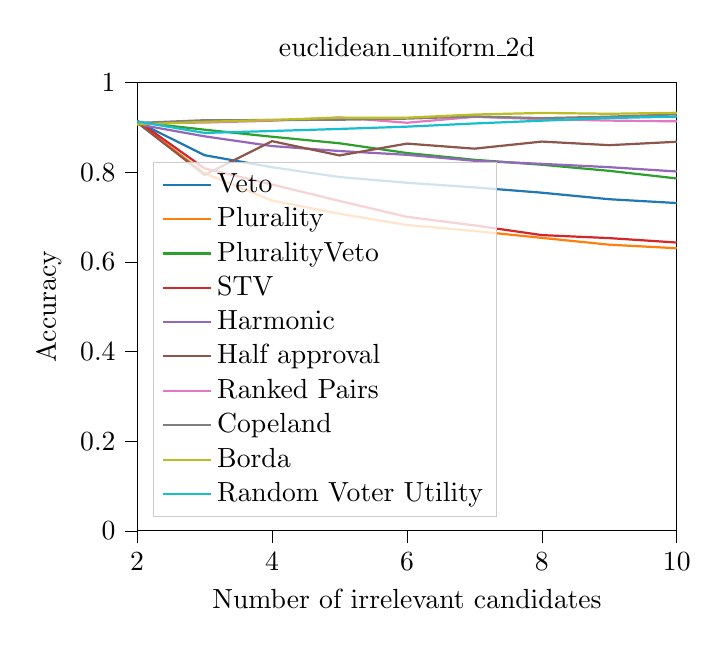
\begin{tikzpicture}

\definecolor{color0}{rgb}{0.12156862745098,0.466666666666667,0.705882352941177}
\definecolor{color1}{rgb}{1,0.498039215686275,0.0549019607843137}
\definecolor{color2}{rgb}{0.172549019607843,0.627450980392157,0.172549019607843}
\definecolor{color3}{rgb}{0.83921568627451,0.152941176470588,0.156862745098039}
\definecolor{color4}{rgb}{0.580392156862745,0.403921568627451,0.741176470588235}
\definecolor{color5}{rgb}{0.549019607843137,0.337254901960784,0.294117647058824}
\definecolor{color6}{rgb}{0.890196078431372,0.466666666666667,0.76078431372549}
\definecolor{color7}{rgb}{0.737254901960784,0.741176470588235,0.133333333333333}
\definecolor{color8}{rgb}{0.0901960784313725,0.745098039215686,0.811764705882353}

\begin{axis}[
legend cell align={left},
legend style={
  fill opacity=0.8,
  draw opacity=1,
  text opacity=1,
  at={(0.03,0.03)},
  anchor=south west,
  draw=white!80!black
},
tick align=outside,
tick pos=left,
title={euclidean\_uniform\_2d},
x grid style={white!69.0196078431373!black},
xlabel={Number of irrelevant candidates},
xmin=2, xmax=10,
xtick style={color=black},
y grid style={white!69.0196078431373!black},
ylabel={Accuracy},
ymin=0, ymax=1,
ytick style={color=black}
]
\addplot [thick, color0]
table {%
2 0.9127
3 0.8378
4 0.811
5 0.7891
6 0.7764
7 0.766
8 0.7542
9 0.7396
10 0.7311
};
\addlegendentry{Veto}
\addplot [thick, color1]
table {%
2 0.9121
3 0.7975
4 0.7367
5 0.7072
6 0.6821
7 0.6687
8 0.6534
9 0.6382
10 0.6303
};
\addlegendentry{Plurality}
\addplot [thick, color2]
table {%
2 0.9118
3 0.8947
4 0.879
5 0.8644
6 0.8427
7 0.8276
8 0.8165
9 0.8029
10 0.786
};
\addlegendentry{PluralityVeto}
\addplot [thick, color3]
table {%
2 0.9151
3 0.8083
4 0.7724
5 0.7358
6 0.7003
7 0.6813
8 0.6596
9 0.6529
10 0.643
};
\addlegendentry{STV}
\addplot [thick, color4]
table {%
2 0.9069
3 0.8799
4 0.8582
5 0.8471
6 0.8387
7 0.8254
8 0.8185
9 0.8111
10 0.8015
};
\addlegendentry{Harmonic}
\addplot [thick, color5]
table {%
2 0.9108
3 0.7939
4 0.8691
5 0.8373
6 0.8637
7 0.8524
8 0.8682
9 0.8602
10 0.8678
};
\addlegendentry{Half approval}
\addplot [thick, color6]
table {%
2 0.9094
3 0.9106
4 0.9148
5 0.922
6 0.9102
7 0.9233
8 0.9183
9 0.915
10 0.9133
};
\addlegendentry{Ranked Pairs}
\addplot [thick, white!49.8039215686275!black]
table {%
2 0.9097
3 0.9159
4 0.9162
5 0.9169
6 0.9194
7 0.9243
8 0.9205
9 0.9238
10 0.9289
};
\addlegendentry{Copeland}
\addplot [thick, color7]
table {%
2 0.9064
3 0.9122
4 0.9165
5 0.9216
6 0.9215
7 0.9285
8 0.9321
9 0.9302
10 0.9324
};
\addlegendentry{Borda}
\addplot [thick, color8]
table {%
2 0.9132
3 0.8875
4 0.8918
5 0.8964
6 0.9015
7 0.9086
8 0.9148
9 0.9207
10 0.9239
};
\addlegendentry{Random Voter Utility}
\end{axis}

\end{tikzpicture}
